% HimaRoad Flood Copilot course report.
% Format source: official CVPR 2026 author kit, commit 12909ae437f6dbc7435069cfdb4ca44c18e6a02f.
\documentclass[10pt,twocolumn,letterpaper]{article}
\usepackage[pagenumbers]{cvpr}
\usepackage{microtype}
\usepackage{booktabs}
\usepackage{multirow}
\usepackage{graphicx}
\usepackage{amsmath}
\usepackage{amssymb}
\usepackage{enumitem}
\usepackage{xspace}
\usepackage{url}
\definecolor{cvprblue}{rgb}{0.21,0.49,0.74}
\usepackage[breaklinks,colorlinks,allcolors=cvprblue]{hyperref}
\newcommand{\CourseAuthors}{
Dishant Kaushik (M24MA2003)\\
Arushi Gandhi (M24MA2001)\\
Aditya Sharma (P25AI0201)\\
Palak Jat (M26MAC006)
}
\newcommand{\CourseAffiliation}{IIT Jodhpur}
\newcommand{\CourseName}{Machine Learning}
\newcommand{\CourseInstructor}{Richa Singh}
\newcommand{\RepositoryURL}{https://github.com/dishant1901-prog/ml\_final\_project.git}


\def\confName{CVPR}
\def\confYear{2026}
\newcommand{\system}{HimaRoad\xspace}
\newcommand{\copilot}{Flood Copilot\xspace}
\newcommand{\unknown}{\textsc{unknown}\xspace}
\setlist{nosep,leftmargin=*}

\title{HimaRoad Flood Copilot: Evidence-Grounded Satellite Flood Mapping,\\
Access Screening, and Bilingual Situation Reporting}
\author{\CourseAuthors\\[2pt]
\CourseAffiliation\\
\CourseName\\
Instructor: \CourseInstructor\\
{\tt\small \RepositoryURL}}

\begin{document}
\maketitle

\begin{abstract}
Rapid flood response in mountain regions requires more than a visually plausible
water mask: responders need provenance, explicit unknown areas, infrastructure
exposure, access scenarios, and concise communication. We present \system, an
open-source prototype that converts free Sentinel-1/2, Copernicus DEM, and
historical OpenStreetMap inputs into versioned hazard evidence, road and
settlement accessibility scenarios, and cited English/Nepali situation reports.
The system enforces same-orbit radar pairing, terrain/coverage masks, immutable
evidence claims, and conservative language that separates satellite overlap from
confirmed damage or closure. A registered UNet achieved 0.766 IoU on its Kuro
Siwo development set but detected 0 of 1,298 labelled new-water pixels in three
once-only Himalayan windows, exposing severe domain shift; consequently, the
showcase defaults to a deterministic radar-change baseline and fails closed when
the authentic checkpoint is absent. In a Trishuli case study, the strict
radar-plus-optical scenario separated an event run (19 potentially cut-off
settlements) from a pre-event control (0), while comparison with Copernicus EMS
landslide products showed low footprint recall (0.012/0.038). These results make
clear that the system is a traceable screening aid, not an operational damage
classifier. We contribute a complete local application, bilingual grounded
reporting, leakage-aware evaluation, and reproducibility artifacts that preserve
both positive and negative findings.
\end{abstract}

\section{Introduction}
Flood and debris-flow response in the Himalaya is an observation problem under
three constraints. First, cloud cover can make optical imagery unavailable when
information is most valuable. Second, synthetic aperture radar (SAR) observes
through cloud but suffers from layover, shadow, speckle, mixed pixels, and
view-angle-dependent change in steep valleys. Third, a hazard pixel alone does
not answer operational questions: which links may be exposed, which settlements
lose mapped access, what remains unobserved, and which facts support a report?

Existing mapping pipelines often optimize a segmentation metric and stop at the
raster. This encourages three unsafe shortcuts: treating unobservable terrain as
negative, treating geometric overlap as confirmed damage, and allowing prose to
outgrow its evidence. \system instead treats each output as a claim with a scope,
source path, checksum, method, and limitations. Its design objective is
\emph{epistemic correctness}: when evidence is missing or incompatible, the
system should say so rather than produce a complete-looking map.

Figure~\ref{fig:architecture} summarizes the end-to-end design. Free provider
inputs pass through strict pairing and observability controls, then two parallel
hazard paths: a reproducible rule detector and an optional registered UNet. The
hazard is intersected with historical infrastructure and propagated through
vehicle/pedestrian graphs. An immutable evidence bundle powers the map, exports,
and a bilingual deterministic copilot.

\begin{figure*}[t]
  \centering
  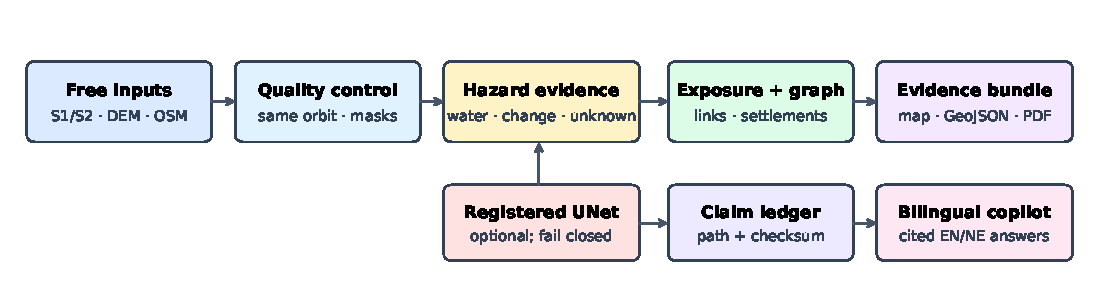
\includegraphics[width=0.98\linewidth]{figures/architecture.pdf}
  \caption{System architecture. Unknown observations remain a first-class state.
  The registered UNet is optional and rejected when its checkpoint or metadata is
  unavailable; downstream reports cite only persisted evidence claims.}
  \label{fig:architecture}
\end{figure*}

The contributions are:
\begin{itemize}
  \item an end-to-end geospatial workflow from provider search to hazard,
  exposure, connectivity, map, GeoJSON/KML, PDF, and bilingual cited answers;
  \item physically constrained SAR processing with same-track pairing,
  observability masks, fixed thresholds, and explicit incomplete states;
  \item graph scenarios that distinguish pre-existing disconnection,
  potentially exposed links, strict corroboration, and worst-case uncertainty;
  \item an evidence-grounded copilot whose EN/NE outputs bind to the same claim
  identifiers and refuse unsupported safe-route or confirmed-damage requests;
  \item an honest domain-shift evaluation, pre-event control, compact
  reproducibility package, and production-oriented local test suite.
\end{itemize}

\section{Related Work and Scientific Basis}
\paragraph{Flood mapping.}
Sentinel-1 supplies calibrated C-band SAR observations independent of daylight
and most cloud conditions~\cite{torres2012sentinel1}. Thresholding a dark
post-event return is common for open-water detection, but terrain, rough water,
vegetation, urban double bounce, and temporal land-cover change complicate the
signal. Operational studies therefore combine change, exclusion masks, terrain,
and post-processing rather than treating a threshold as universally valid
\cite{twele2016sentinel,twele2019sen1flood}. Sentinel-2 provides multispectral
corroboration when cloud permits~\cite{drusch2012sentinel2}. Our system maintains
radar and optical evidence separately so corroboration can tighten an access
scenario without silently rewriting the radar result.

\paragraph{Learned segmentation and domain shift.}
U-Net's encoder--decoder structure is a strong dense-prediction baseline
\cite{ronneberger2015unet}. Sen1Floods11 established a geographically distributed
Sentinel-1 flood benchmark~\cite{bonafilia2020sen1floods11}; Kuro Siwo emphasizes
multi-temporal flood mapping and includes quality-aware labels
\cite{bountos2024kurosiwo}. However, lowland benchmarks do not guarantee transfer
to narrow Himalayan valleys. Rather than hide this gap, we report the selected
model's development result alongside a once-only held-out failure.

\paragraph{Infrastructure and accessibility.}
OpenStreetMap (OSM) provides global volunteered roads, paths, buildings and
facilities~\cite{haklay2010osm}. Network reachability can expose where a suspected
closure changes access, but the answer is only as complete as the graph and its
tags. We therefore preserve pedestrian and vehicle modes, evaluate pre-event
reachability, and phrase every result as a scenario rather than a verified safe
route. DEM-derived drainage context and HAND-like terrain measures provide
hydrologic context but are not treated as observations of water
\cite{nobre2011hand}.

\paragraph{Evidence-grounded reporting.}
The reporting problem is distinct from open-ended text generation: numerical
claims must remain traceable across a map, API, and two languages. We use a
deterministic claim ledger and bounded question templates. This resembles data
lineage more than free-form question answering: values are rendered only after
their source file, JSON path, method and checksum pass validation.

\section{System Design}
\subsection{Inputs, pairing, and spatial grid}
The request contains an event date and bounded area. The live CDSE adapter
searches Sentinel-1 scenes before and after the event and accepts only a
same-relative-orbit pair. Cross-orbit comparisons are rejected because
look-direction and incidence changes can dominate the terrain signal. An area
larger than 600~km$^2$, a pre-Sentinel-1 date, missing scenes, or an exhausted
time budget produces a structured \texttt{incomplete} run rather than partial
success.

Accepted SAR bands are projected to a north-up 20~m UTM grid. Every date has a
provider validity mask; the common analysis support is their intersection with
the area of interest. Sentinel-2 L2A is aligned independently and cloud masked.
Copernicus GLO-30 supplies slope, a drainage-relative height layer, and an
optional D8 flow path. Infrastructure is requested from the ohsome API at 00:00
UTC on the day before the event, preventing post-event edits from becoming
implicit evidence.

\subsection{Hazard and observability}
Let $S_{pre}$ be the per-pixel median of valid pre-event VV observations in dB
and $S_{post}$ the post-event VV. The baseline candidate is
\begin{equation}
W = [S_{post}<-16] \land [S_{pre}-S_{post}\ge3].
\end{equation}
Permanent-water candidates ($S_{pre}<-20$~dB), slopes above $12^\circ$, invalid
support, and connected components below 1,600~m$^2$ are removed. Fixed values are
configuration, not universally optimal parameters. A standardized two-sided
change score also marks disturbance, while brightening in a valley-bottom
corridor becomes \texttt{possible\_debris}. The latter is explicitly unvalidated
rule evidence and may represent scour, vegetation, construction, geometric
effects, or landslide debris.

Radar layover and shadow are estimated along DEM range lines and combined with
provider masks. Such pixels become \unknown rather than no-change. This
three-state discipline propagates to road links and summaries. HAND is a soft
context flag, never a substitute water observation. Optical water/change indices
remain separate evidence so missing cloud-free imagery cannot erase a radar
candidate.

\subsection{Exposure and access scenarios}
Roads are segmented and intersected with hazard and observability polygons.
Links receive mutually exclusive evidence categories such as likely impact,
observed change, no detected change, or unobservable. Buildings are counted as
potentially exposed only through geometric overlap. Neither category asserts
physical damage or closure.

Vehicle and pedestrian directed graphs are built from OSM tags. Settlements come
from place nodes and spatially clustered buildings; destinations include towns
and health facilities. Pre-event connectivity is evaluated first to avoid
calling an already disconnected settlement newly cut off. Four counterfactual
scenarios remove: (1) independent confirmed closures; (2) confirmed plus observed
or likely-impact links; (3) a strict subset with radar and optical corroboration;
and (4) broad plus possible-impact, unobservable, and operationally unknown
links. The strict scenario is the headline in the case study; broad and
worst-case outputs are sensitivity bounds.

\subsection{Immutable evidence and bilingual copilot}
Each completed run is normalized into a bounded bundle. Claims contain a stable
identifier, value/unit, source file, source path, method, observation status and
SHA256. The serving layer validates these bindings before a question is
available. Predefined query families cover impact summary, potentially affected
roads/buildings, cut-off settlements, facilities, uncertainty, provenance,
methods, and routes. EN and NE renderers consume identical claim IDs. Requests
for safe routes, confirmed collapse, casualties, causation, or unavailable
precision are refused or reformulated with limitations.

The app uses FastAPI and a single-page map interface. Prepared evidence is
cached with bounded memory; expensive preparation can run in a local worker.
Basic authentication, localhost-first defaults, security headers, path
containment, rate/size limits, health endpoints and graceful degraded states
support an internal showcase. Figure~\ref{fig:ui} shows the validated desktop
interface.

\subsection{Run contract and provenance}
A run is a directory with an explicit schema version rather than an informal
collection of map files. Its manifest records request bounds/date, provider item
identifiers, acquisition timestamps, orbit information, coordinate reference
system, pixel transform, detector and preprocessing versions, thresholds,
software commit, per-file checksums, completion state and limitations. The
summary JSON is derived from the same bounded layers that are exported. A bundle
builder verifies paths and hashes before making a run available to the copilot;
later modification invalidates the prepared evidence.

This contract prevents several common reproducibility failures. A cached raster
cannot silently migrate between requests because its request fingerprint and
source identifiers are checked. Absolute workstation paths are not published in
portable artifacts. Run identifiers are treated as untrusted input and resolved
inside configured roots. Schema adapters can read older bundles, but cannot
invent fields that the older producer did not observe. If a field is absent, the
claim status remains unavailable rather than receiving a modern default.

Provenance also preserves temporal semantics. ``Event date'' is a request
boundary, not the unknown physical onset time. Observation time is taken from
the satellite item, and OSM snapshot time is reported separately. The Trishuli
primary radar post scene, for example, was acquired about 60.4 hours after the
event-date boundary. Reports expose that lag because rapid-onset hazards can
change substantially between the event and the next valid pass.

\subsection{Unknown-state algebra}
Binary map arithmetic easily converts missing observations into false negatives.
We avoid this by carrying support masks beside values. For a pixel $i$, a hazard
predicate $h_i$ is evaluated only when observation support $o_i=1$; otherwise
its state is unknown. For a road segment $e$ intersecting pixel set $P_e$, we
separate observed hazard, observed no-change, and unobservable fractions:
\begin{align}
q_e^+ &= |\{i\in P_e:o_i=1,h_i=1\}|/|P_e|,\\
q_e^0 &= |\{i\in P_e:o_i=1,h_i=0\}|/|P_e|,\\
q_e^? &= |\{i\in P_e:o_i=0\}|/|P_e|.
\end{align}
These quantities are not normalized over observed pixels alone, so a mostly
hidden link cannot appear confidently negative because of one visible pixel.
Graph scenarios then decide explicitly whether unknown links remain or are
removed; the worst-case scenario removes them, whereas the strict scenario does
not turn them into evidence. This distinction explains why uncertainty counts
can be large even when the final water mask is empty.

\begin{figure}[t]
  \centering
  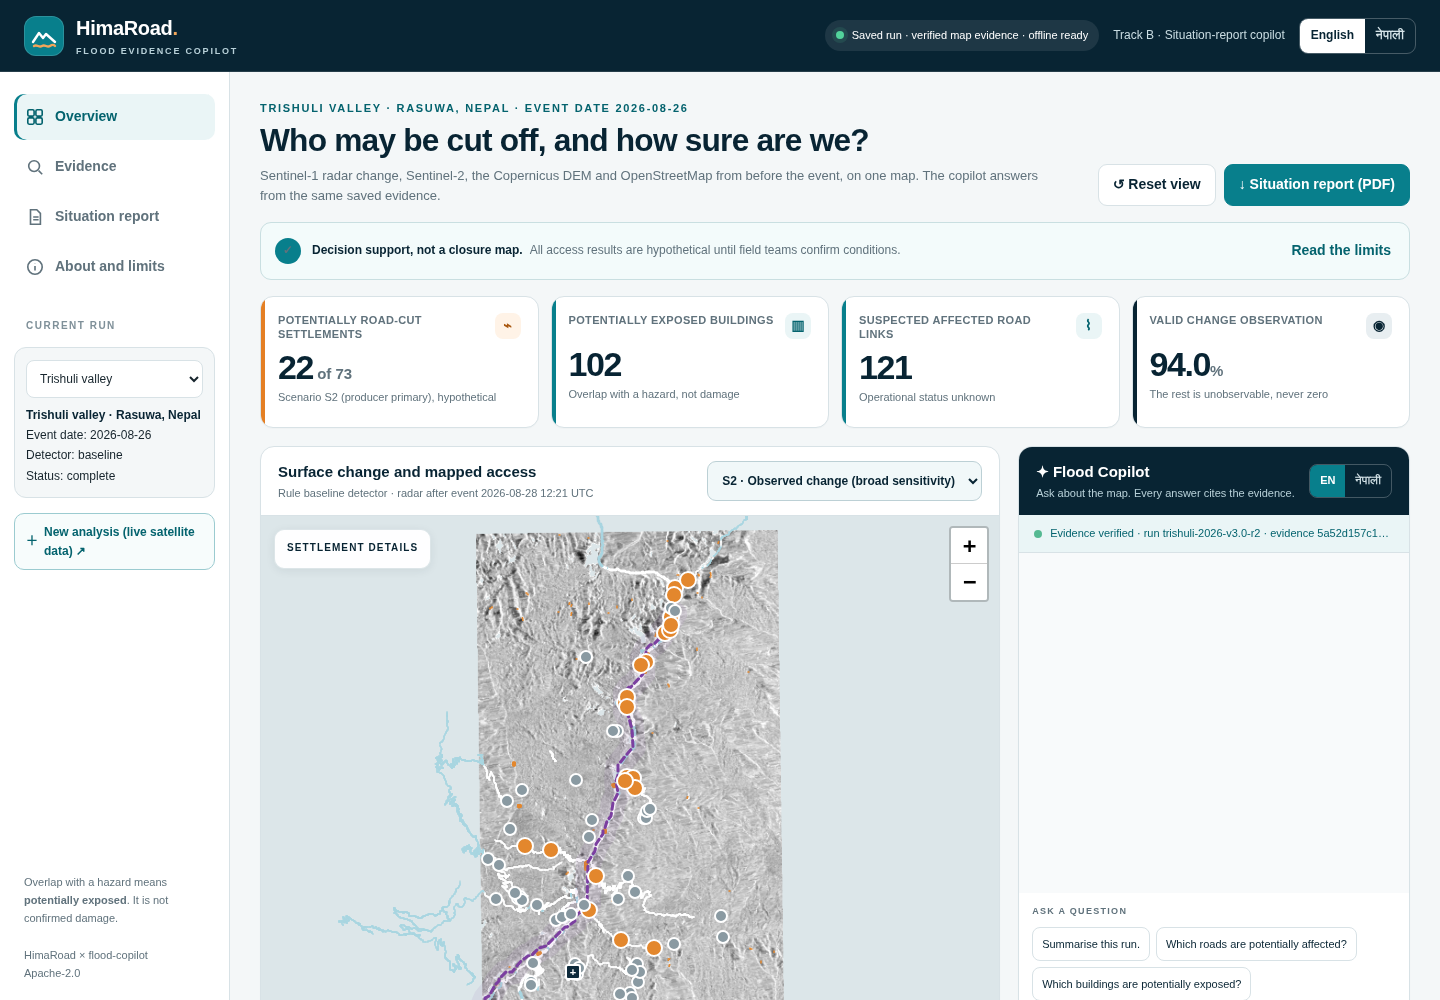
\includegraphics[width=\linewidth]{figures/dashboard.png}
  \caption{Polished local dashboard: hazard/access map, evidence status, language
  switch and grounded copilot share one interface.}
  \label{fig:ui}
\end{figure}

\section{Registered Model and Evaluation Protocol}
\subsection{UNet configuration}
The historical registered model is a four-channel UNet (pre/post VV/VH), base
width 32 and depth 4. Inputs are clipped/normalized dB bands on the 20~m UTM
grid. Training recorded 310 Kuro Siwo chips from Houston, Togo and Peru; 134
development chips came from Larkana and Illinois. Four registered variants were
trained from scratch for 30 epochs with seed 42, BCE+Dice loss, AdamW at
$3\times10^{-4}$, batch size four, and deterministic event/region separation.
The lowest development loss selected the architecture; temperature 1.4940904 and
threshold 0.57 were fixed on development data subject to a 0.80 precision floor.

The dataset loader enforces invariants before reading a chip: train/dev/test
events and regions cannot overlap; Nepal, mountain, and unknown-terrain events
cannot enter training; reference-map path tokens are refused; files must remain
inside an explicit dataset root; and each selected file requires frozen size and
SHA256. Model loading similarly verifies preprocessing ID, calibration split,
metadata, tiling, expected hash, and a synthetic-weight flag.

\subsection{What is and is not reproducible}
The configured checkpoint SHA256 is \texttt{3ed60130\ldots a7098e5}; the
complete digest is preserved in the checkpoint register.
The weights, frozen v2 split, original source labels and complete historical
training entry point are absent from both this checkout and its public history.
Accordingly, we do not claim to have rerun training or independently reproduced
the checkpoint. The recorded scores are historical artifacts, and the local
application defaults to the rule detector. This boundary is preferable to
training on reconstructed splits after seeing the test results.

\subsection{Evaluation discipline}
Development events selected both architecture and operating point; their scores
are not blind accuracy. A once-only Himalayan check used valley-enriched
128$\times$128 windows from Teesta 2023, Melamchi 2021 and Chamoli 2021. Two
reviewers labelled independently and adjudicated. No threshold, model, or
checkpoint changed afterward. Published Copernicus EMS products were opened only
after a fresh case-study run was frozen and are isolated from inference, tuning,
and model selection. A leakage scan records this separation.

\subsection{Metrics and interpretation}
For eligible observed pixels, we report precision $TP/(TP+FP)$, recall
$TP/(TP+FN)$, intersection-over-union $TP/(TP+FP+FN)$, and F1. A denominator of
zero yields unavailable, not zero. Development micro-metrics pool pixels and can
be dominated by a large event, so per-event values and sample counts accompany
the aggregate. The Himalayan test reports raw confusion counts because the small
number of positive pixels makes percentages deceptively precise.

The EMS reference is not a pixel-equivalent water ground truth. Its grading
products use very-high-resolution optical interpretation and describe landslide
footprints/transport damage, while \system measures 20~m SAR/optical change.
Therefore we compute positive-footprint area recall and matched transport-feature
recall within shared coverage, not water IoU or unrestricted background
specificity. Unassessed areas never become reliable negatives. For infrastructure
matching, a buffered candidate must have appreciable linear overlap; a nearby
crossing alone is insufficient. Connectivity is not scored from imagery because
an independent closure observation is required to validate removal of a graph
edge.

The pre-event control asks a different question: does the configured pipeline
produce similarly strong access alarms when all selected observations predate the
event? It is not a random negative sample and cannot estimate a population false
alarm rate. It is nevertheless valuable for detecting a non-discriminative
headline scenario within the same AOI and network.

\section{Experiments and Results}
\subsection{Model development versus Himalayan transfer}
Table~\ref{tab:model} and Figure~\ref{fig:model} expose the central negative
result. On 1,167,702 valid development pixels, the selected UNet improved IoU
from 0.610 to 0.766 and F1 from 0.758 to 0.867, trading precision for recall.
Across the Himalayan primary windows, however, it predicted no positives and
detected 0/1,298 labelled new-water pixels. The baseline found 24 true positives
with pooled precision 0.828, recall 0.018 and IoU 0.018. Thus neither approach is
an accurate Himalayan flood segmenter, and the learned development gain does not
transfer.

\begin{table}[t]
\centering
\caption{Kuro Siwo development metrics. This split selected the model and is not
an independent generalization estimate.}
\label{tab:model}
\small
\begin{tabular}{lrrrr}
\toprule
Method & Prec. & Recall & IoU & F1 \\
\midrule
Rule baseline & .8835 & .6629 & .6096 & .7575 \\
Selected UNet & .8008 & .9457 & .7656 & .8672 \\
\bottomrule
\end{tabular}
\end{table}

\begin{figure}[t]
  \centering
  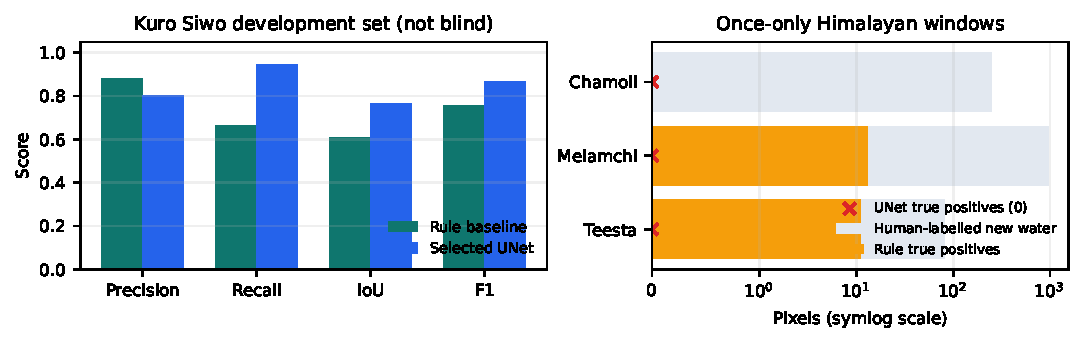
\includegraphics[width=\linewidth]{figures/model-results.pdf}
  \caption{Left: model-selection evidence. Right: labelled positives and true
  positives on once-only Himalayan windows; the UNet true-positive count is zero
  for every event.}
  \label{fig:model}
\end{figure}

The windows are deliberately valley enriched and small, so they are not a
regional prevalence sample. Inter-reviewer agreement was low for Teesta and
Chamoli. Those limitations widen uncertainty; they do not justify replacing the
observed zero-recall result with the development score.

\subsection{Trishuli case study}
The authenticated 2 November reproduction used the Bhote Koshi--Trishuli area
for 26 August 2026 and acquired same-track Sentinel-1, Sentinel-2, DEM/HAND and
pre-event OSM from configured providers. The frozen output contains zero final
flood pixels, 474 disturbance pixels, 109 possible-debris pixels and 22 broad
potential cut-offs. A zero water layer means no pixels met the configured rule in
observable support; it does not establish no flood.

Copernicus EMSR927 describes this activation's observed-event class as
landslide, so water IoU is inapplicable. A checking-only comparison measured
positive-footprint recall 0.012 for AOI01 Syapru Besi and 0.038 for AOI02 Timure.
The system recalled affected transport grades on 6/19 and 7/13 features,
respectively, while flagging 0/8 AOI01 ``no visible damage'' references. Most
AOI01 misses were observed with no detected change; most AOI02 misses were fully
or partly unobservable. This is a detection failure, not merely a coverage gap.

A matched pre-event control used otherwise identical processing dated 10 August.
The broad scenario was weakly discriminative (22 event versus 19 control
cut-offs), whereas the strict radar-plus-optical scenario produced 19 versus 0
cut-offs and 16 versus 0 likely-impact links (Figure~\ref{fig:control}). This
supports using strict corroboration as the headline for this case, not a claim of
universal accuracy. A roughly 50-day optical gap and a single control leave
seasonal change and selection effects unresolved.

\begin{figure}[t]
  \centering
  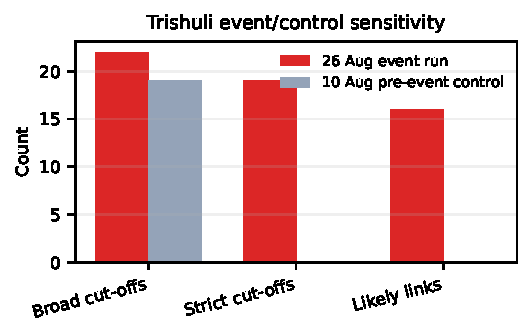
\includegraphics[width=\linewidth]{figures/case-study.pdf}
  \caption{Event/control comparison. Broad graph sensitivity remains high in the
  control; strict corroboration separates this pair but is not field truth.}
  \label{fig:control}
\end{figure}

\subsection{Robustness, latency, and reporting}
Six unlabelled public AOIs tested failure behavior under a 180~s budget rather
than accuracy. Lokoja and Lismore completed; Valencia timed out; Porto Alegre had
no same-track pair; Manila predates Sentinel-1; and an oversized Germany request
was rejected before download. Every non-completion returned a specific reason.
On a 600~km$^2$ real input (1,433,870 observable pixels), recorded warm detector
median was 4.929~s on CPU and 1.702~s on GPU, excluding acquisition, graph and
export stages.

The prepared copilot validated 32 predefined cases (eight query families, two
languages, two areas) with exact EN/NE claim-ID parity. Current Trishuli
verification checked 62,260 evidence claims. Individual prepared-answer latency
was 0.628--0.909~s; one-page EN and NE PDFs each took about 24~s. These are local
measurements, not service-level guarantees. Full evidence export peaked near
3.68~GiB RSS, motivating bounded preparation and gzip artifacts.

\subsection{Error analysis}
The failures have different causes and remediation paths. The UNet's zero
Himalayan recall is consistent with covariate and concept shift: lowland training
events contain broad, relatively smooth open water, whereas valley floods can be
narrow, turbulent, debris laden, vegetated, geometrically distorted, and only a
few 20~m pixels wide. Calibration at a development precision floor further makes
the deployed operating point conservative. Lowering the threshold after viewing
the Himalayan test would contaminate the once-only evaluation and is therefore
not attempted.

The rule detector misses for overlapping reasons but has inspectable decisions.
In AOI01, most missed affected transport features were in support classified as
observed with no detected change; this points to insufficient signal/threshold or
resolution rather than masking. In AOI02, most misses were fully or partially
unobservable, pointing to SAR geometry and motivating alternative orbits, optical
data, field reports, or higher-resolution sensors. These categories matter:
loosening a backscatter threshold cannot recover a shadowed road, while a new
sensor cannot by itself fix label-definition mismatch.

The broad graph scenario's 22-versus-19 event/control result shows amplification:
even a small number of suspected links can disconnect many destinations when the
network has bridges or single-access corridors. Graph impact is therefore not an
independent confirmation of the hazard detector. The strict scenario reduces
that amplification by requiring optical corroboration, but its apparent
separation may also reflect cloud/season timing. Prospective multi-event controls
are necessary before treating either scenario as calibrated.

The robustness drills also distinguish expected abstention from software failure.
Rejecting an oversized AOI, a pre-mission date, or an incompatible orbit pair is
correct behavior. A timeout in dense Valencia indicates a performance bottleneck:
recorded diagnostics attributed most time to infrastructure exposure, graph
construction and export. Spatial indexing, graph tiling, streaming export and
provider-side caching are higher-priority improvements than optimizing the
already faster pixel detector.

\section{Reliability and Reproducibility}
\subsection{Testing and failure containment}
The repository includes unit and integration tests for geospatial alignment,
unknown-state propagation, event/region leakage, bundle integrity, graph
semantics, evidence claim binding, bilingual parity, report pagination, refusal
behavior, API contracts, authentication, path containment, caching and worker
operations. A local CI script runs compile checks, the test suite, secret scans,
scientific validation, offline validation, package verification, and dependency
audits. Health endpoints distinguish liveness from readiness; a missing prepared
copilot run leaves the map available and returns a bounded error instead of an
uncited answer.

Security defaults fit an internal prototype: localhost binding, generated basic
auth credentials, no secrets in the repository, request and response limits,
safe-path validation, immutable evidence paths, security headers, dependency
pinning and a non-root container. This is not equivalent to a production security
review. Internet-exposed deployment would additionally require managed identity,
TLS termination, centralized secrets, rate limiting, monitoring, backups,
provider quotas and incident procedures.

\subsection{Readiness matrix}
Table~\ref{tab:readiness} separates demonstrated engineering properties from
open production requirements. ``Verified'' means an automated local artifact or
test exists; it does not imply independent certification.

\begin{table}[t]
\centering
\caption{Readiness assessment at submission time.}
\label{tab:readiness}
\small
\setlength{\tabcolsep}{3pt}
\begin{tabular}{@{}p{0.34\linewidth}p{0.20\linewidth}p{0.40\linewidth}@{}}
\toprule
Capability & State & Evidence / next gate \\
\midrule
Offline pipeline contracts & Verified & unit/integration tests \\
Evidence-bound EN/NE answers & Verified & claim-ID parity checks \\
Local authenticated showcase & Verified & browser/API regression \\
Dependency and secret hygiene & Verified & lock/export + scans \\
Himalayan flood accuracy & Failed & new prospective labels \\
Model checkpoint reproduction & Blocked & authentic weights/splits \\
Internet security/operations & Not reviewed & managed deployment review \\
Emergency decision authority & Out of scope & field/agency validation \\
\bottomrule
\end{tabular}
\end{table}

\subsection{Threats to validity}
\emph{Internal validity} is limited by unavailable historical training assets and
manual labels; recorded model results cannot be freshly audited end to end.
Checksums protect artifacts that exist but do not prove the original measurement
procedure. \emph{Construct validity} is limited because SAR change, EMS landslide
interpretation, physical damage, closure and accessibility are related but
different constructs. We avoid merging them into one accuracy number.
\emph{External validity} is limited by three small Himalayan windows, one
case-study AOI/control and unlabelled robustness drills. \emph{Statistical
conclusion validity} is limited by event dependence, severe class imbalance and
few independent events; pixel counts are not equivalent to independent samples.

Mitigations include frozen event-level splits, no Nepal/mountain training events,
raw confusion counts, per-event reporting, positive-only EMS interpretation,
explicit unavailable metrics, and refusal to tune on consumed test events. The
remaining risks require new data and prospective design, not additional decimals
on current scores.

\subsection{Reproducibility package}
The repository pins Python 3.12 dependencies in \texttt{uv.lock} and exports
\texttt{requirements.txt}, \texttt{requirements-model.txt}, and
\texttt{environment.yml}. \texttt{REPRODUCIBILITY.md} defines clean setup,
offline checks, external-data boundaries and report construction.
\texttt{DATASETS.md} records each external input and expected layout;
\texttt{CHECKPOINTS.md} records the missing checkpoint identity without implying
availability. Machine-readable receipts contain hashes, versions, test results,
page count, and Git history. Large provider data, validation archives,
credentials, and generated runs are ignored rather than silently vendored.

The CVPR PDF itself is built from the official 2026 author kit pinned to commit
\texttt{12909ae437f6dbc7435069cfdb4ca44c18e6a02f}. A local Tectonic build script
regenerates figures, compiles the source, rejects unresolved references, and
requires exactly eight pages. The final repository commit hash and timestamp are
obtained directly from Git, not typed into the paper, avoiding a self-referential
manifest.

Repository history is part of the artifact: Git retains author, full commit hash,
parent and ISO timestamp, while the verification script exports those fields into
a machine-readable receipt. The final commit cannot truthfully list its own hash
inside itself, so evaluators are instructed to inspect \texttt{git log} (or the
hosting service) for the authoritative final value. This avoids fabricated or
stale commit metadata.

\section{Limitations, Ethics, and Deployment Scope}
\paragraph{Scientific limitations.}
The UNet fails on the held-out Himalayan windows; the rule baseline also has very
low recall. The debris class is unvalidated. SAR cannot reliably observe every
steep valley surface, optical gaps are common, and 20~m pixels miss narrow
features. EMS comparison uses positive-only reference footprints and different
sensor/resolution semantics. One control is insufficient to estimate a false
positive rate. Human labels and the historical training package are unavailable,
preventing independent checkpoint reproduction.

\paragraph{Operational limitations.}
Potential exposure is not confirmed damage, operational status, or closure.
Graph removal is a counterfactual accessibility scenario, and a mapped path is
not a safe route. OSM can be incomplete or mistagged. Satellite acquisition is
post-event and cannot provide minute-scale early warning. Cause, casualties,
depth, velocity, arrival time and structural safety are outside scope. Outputs
require independent local inspection and authoritative emergency information.

\paragraph{Language and human factors.}
The Nepali templates passed terminology inventory and claim-parity checks, but
automated glyph and binding validation is not a substitute for community review
in every dialect and operational setting. Warnings, unknown states and evidence
timestamps remain visible in both languages. The interface limits feature counts
for responsiveness while preserving full exports as authoritative artifacts.

\paragraph{Deployment decision.}
The system is suitable for a localhost internal demonstration and research
reproduction. It is not ready to make autonomous emergency decisions or to be
treated as a reliable production damage product. A production path requires new
representative Himalayan labels, prospective multi-event evaluation, calibrated
uncertainty, authenticated checkpoint release, load/security testing, monitored
data-provider contracts and acceptance review by disaster-response experts.

\subsection{Prospective validation path}
The next scientific milestone should be designed before collecting outcomes. We
would register event-level train, development and test regions; prohibit spatial
or temporal overlap; and stratify Himalayan events by valley width, land cover,
snow, flood mechanism, orbit geometry and season. Labels should include open
water, permanent water, debris/turbid water, invalid observation and ambiguous
pixels, with independent reviewers blind to model output. The primary endpoint
would be event-macro IoU/recall within observable support, accompanied by raw
confusion counts and bootstrap intervals over events rather than pixels.

High-precision and high-recall operating points must be frozen on development
data before opening test labels. Comparators should include the fixed rule, an
adaptive threshold, the authentic registered UNet if recovered, and a retrained
temporal model; ablations should report both accuracy and abstention/coverage.
Infrastructure validation additionally needs timestamped confirmed-open/closed
links, while field partners review graph modes, warnings and Nepali wording.
Signed artifacts, load/soak, provider-failure, security and rollback tests are
additional gates beyond scientific accuracy.

\section{Conclusion}
\system demonstrates that a useful flood-mapping project is not defined only by
a segmentation network. The larger contribution is a chain of controlled
evidence: compatible satellite pairing, explicit observability, conservative
exposure language, preconditioned access scenarios, immutable claim binding and
bilingual delivery. The evaluation also demonstrates the value of publishing a
negative transfer result. A UNet that looks strong on development data can fail
completely in Himalayan valleys, and a visually polished map cannot repair that
scientific gap. By defaulting to reproducible rules, refusing unavailable model
artifacts, preserving unknowns, and exposing limitations at the point of use,
the project provides a credible base for future data collection and prospective
validation without overstating present capability.

{\small
\bibliographystyle{ieeenat_fullname}
\bibliography{main}
}

\end{document}
